% Study flow of the final paper: what each version ran, on which cases, and why the next one followed. TikZ; compile with pdflatex.
\documentclass[tikz,border=3pt]{standalone}
\usepackage[T1]{fontenc}
\usepackage[scaled=0.92]{helvet}
\renewcommand{\familydefault}{\sfdefault}
\usetikzlibrary{arrows.meta,calc,positioning}
\definecolor{vfill}{HTML}{FFFFFF}\definecolor{vline}{HTML}{4D4D4D}
\definecolor{pilotc}{HTML}{E69F00}\definecolor{mainc}{HTML}{0072B2}\definecolor{confc}{HTML}{009E73}
\definecolor{ragfill}{HTML}{DCEEFB}
\hyphenpenalty=10000\exhyphenpenalty=10000
\begin{document}
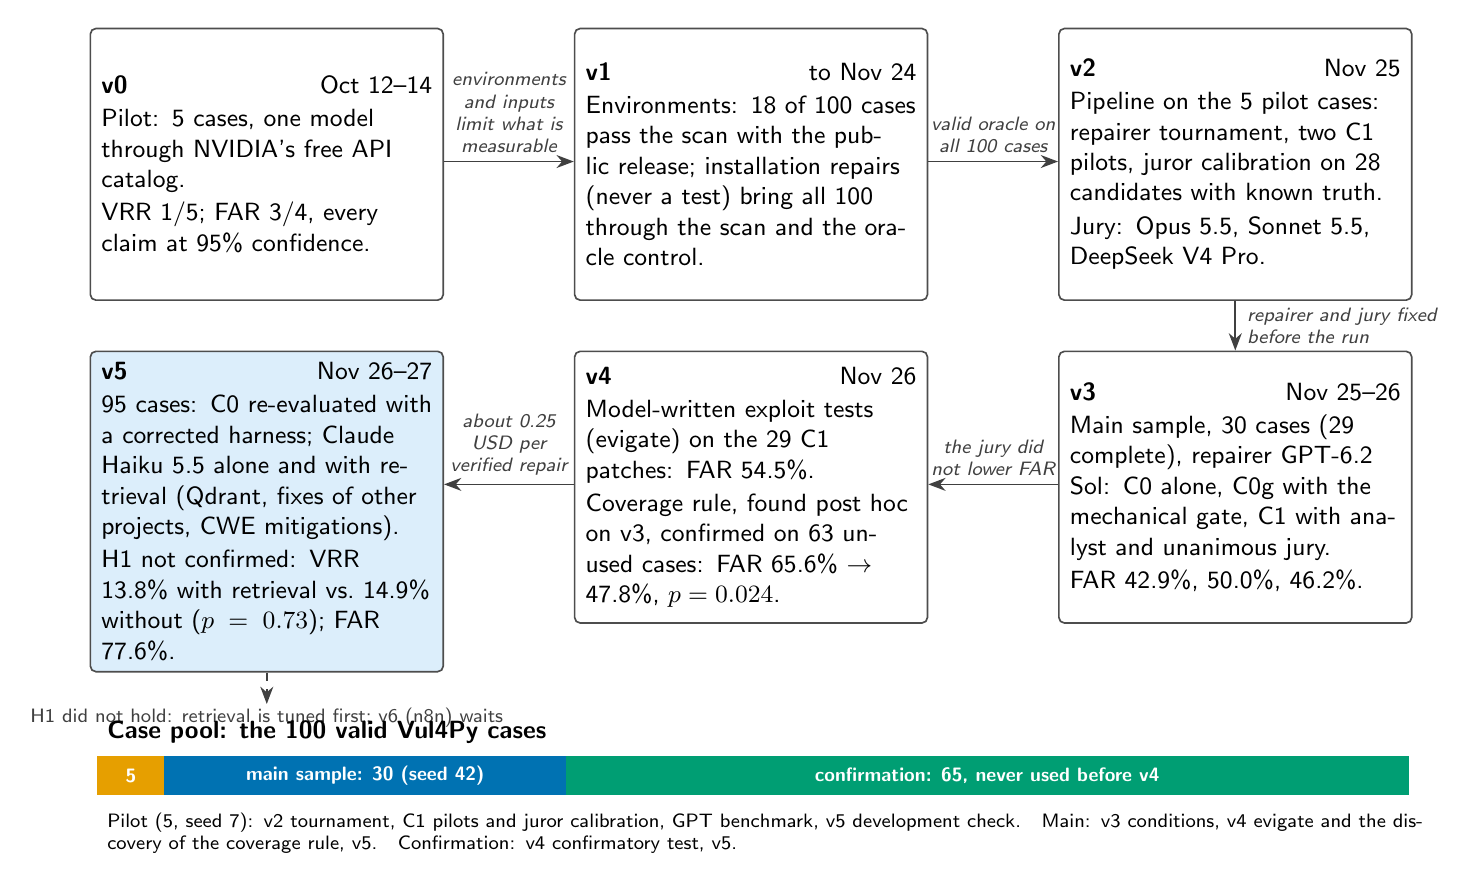
\begin{tikzpicture}[
  font=\small,
  ver/.style={draw=vline, fill=vfill, rounded corners=2pt, align=left, text width=4.2cm, minimum height=3.45cm, inner sep=4pt, line width=0.6pt, anchor=north},
  head/.style={font=\small\bfseries},
  arr/.style={-{Stealth[length=2.2mm]}, line width=0.6pt, color=black!75},
  why/.style={font=\scriptsize\itshape, align=center, text width=1.65cm, inner sep=1pt},
  tag/.style={font=\scriptsize\bfseries, text=white, rounded corners=1pt, inner sep=1.5pt}
]
% ------------------------------------------------------------ row 1
\node[ver] (v0) at (2.35,0) {{\bfseries v0} \hfill Oct 12--14\\[1pt]
  Pilot: 5 cases, one model through NVIDIA's free API catalog.\\[1pt]
  VRR 1/5; FAR 3/4, every claim at 95\% confidence.};
\node[ver] (v1) at (8.5,0) {{\bfseries v1} \hfill to Nov 24\\[1pt]
  Environments: 18 of 100 cases pass the scan with the public release; installation repairs (never a test) bring all 100 through the scan and the oracle control.};
\node[ver] (v2) at (14.65,0) {{\bfseries v2} \hfill Nov 25\\[1pt]
  Pipeline on the 5 pilot cases: repairer tournament, two C1 pilots, juror calibration on 28 candidates with known truth.\\[1pt]
  Jury: Opus 5.5, Sonnet 5.5, DeepSeek V4 Pro.};
% ------------------------------------------------------------ row 2
\node[ver] (v3) at (14.65,-4.1) {{\bfseries v3} \hfill Nov 25--26\\[1pt]
  Main sample, 30 cases (29 complete), repairer GPT-6.2 Sol: C0 alone, C0g with the mechanical gate, C1 with analyst and unanimous jury.\\[1pt]
  FAR 42.9\%, 50.0\%, 46.2\%.};
\node[ver] (v4) at (8.5,-4.1) {{\bfseries v4} \hfill Nov 26\\[1pt]
  Model-written exploit tests (evigate) on the 29 C1 patches: FAR 54.5\%.\\[1pt]
  Coverage rule, found post hoc on v3, confirmed on 63 unused cases: FAR 65.6\% $\to$ 47.8\%, $p=0.024$.};
\node[ver, fill=ragfill] (v5) at (2.35,-4.1) {{\bfseries v5} \hfill Nov 26--27\\[1pt]
  95 cases: C0 re-evaluated with a corrected harness; Claude Haiku 5.5 alone and with retrieval (Qdrant, fixes of other projects, CWE mitigations).\\[1pt]
  H1 not confirmed: VRR 13.8\% with retrieval vs.\ 14.9\% without ($p=0.73$); FAR 77.6\%.};
% ------------------------------------------------------------ arrows with reasons
\draw[arr] (v0.east |- 0,-1.7) -- node[why, above=2pt] {environments and inputs limit what is measurable} (v1.west |- 0,-1.7);
\draw[arr] (v1.east |- 0,-1.7) -- node[why, above=2pt] {valid oracle on all 100 cases} (v2.west |- 0,-1.7);
\draw[arr] (v2.south) -- node[why, right=3pt, text width=2.6cm, align=left] {repairer and jury fixed before the run} (v3.north);
\draw[arr] (v3.west |- 0,-5.8) -- node[why, above=2pt] {the jury did not lower FAR} (v4.east |- 0,-5.8);
\draw[arr] (v4.west |- 0,-5.8) -- node[why, above=2pt] {about 0.25 USD per verified repair} (v5.east |- 0,-5.8);
\draw[arr, dashed] (v5.south) -- ++(0,-0.4) node[below, font=\scriptsize, align=left, inner sep=1pt] {H1 did not hold: retrieval is tuned first; v6 (n8n) waits};
% ------------------------------------------------------------ case pool
\begin{scope}[shift={(0,-9.5)}]
  \node[font=\small\bfseries, anchor=west] at (0.2,0.55) {Case pool: the 100 valid Vul4Py cases};
  \fill[pilotc] (0.2,-0.25) rectangle ++(0.85,0.5);
  \fill[mainc] (1.05,-0.25) rectangle ++(5.1,0.5);
  \fill[confc] (6.15,-0.25) rectangle ++(10.7,0.5);
  \node[tag] at (0.625,0) {5};
  \node[tag] at (3.6,0) {main sample: 30 (seed 42)};
  \node[tag] at (11.5,0) {confirmation: 65, never used before v4};
  \node[font=\scriptsize, anchor=north west, align=left, text width=16.8cm] at (0.2,-0.35)
    {Pilot (5, seed 7): v2 tournament, C1 pilots and juror calibration, GPT benchmark, v5 development check.\quad
     Main: v3 conditions, v4 evigate and the discovery of the coverage rule, v5.\quad
     Confirmation: v4 confirmatory test, v5.};
\end{scope}
\end{tikzpicture}
\end{document}
